% Drawing 154/03-3 -- folder 154, batch 03, archive page 46 (PDF page 47).
% Transcription: figure au milieu de la colonne : deux droites vertes (horizontale et verticale) traversées de pseudo-droites orange qui s'entrecroisent, un point de concours en pointillé orange
% Kind: two green lines crossed by orange pseudolines. Method 2 (schematic redraw from the facsimile). Status: ok.
% Notes: Right column: a horizontal green line and two vertical green lines crossed by orange pseudolines that cross one another; at the crossing of the horizontal line with the right-hand vertical, a point of concurrence drawn in dotted orange. The transcription speaks of two green lines; the page has one horizontal and two vertical ones. The large band figure at the head of the left column is described in a \note, not by this mark.
% Coordinates: 1 unit = 1 mm = 1/100 of the crop width (bbox in page fractions: [0.76, 0.319, 0.909, 0.38]).
% Redrawn by Claude (claude-opus-5-5), issue #73, 2026-11-07; not checked by a human; not compiled (no TeX in the session).
% Revised by Claude (claude-opus-5-5) 2026-11-09 (issue #128) after Michel's check: vertices snapped to exact intersections (drawn points on their lines, meeting ends on the stroke they meet, near-concurrent lines through one computed point, curve ends on their rim); labels at \small as in folder 80 batch 3. Status: ok.
% Rights: reproduces part of the work -- behind RENDER_TRANSCRIPTS, never published by itself.
\documentclass[tikz,border=3pt]{standalone}
\usepackage{amsmath,amssymb}
\usetikzlibrary{patterns,arrows.meta}
\tikzset{Or/.style={orange!90!black}, Ye/.style={yellow!80!orange}, Lg/.style={green!60!black!70}, Dg/.style={green!45!black}, Br/.style={brown!80!black}, Rd/.style={red!85!black}, Bl/.style={blue!70!black}, Gy/.style={black!40}, pencil/.style={black!45}, struck/.style={black!35}, mark/.style={circle,draw,inner sep=1.3pt}, pt/.style={circle,fill,inner sep=0.9pt}, opt/.style={circle,draw,fill=white,inner sep=1.1pt}}
\colorlet{Or}{orange!90!black}\colorlet{Ye}{yellow!80!orange}\colorlet{Lg}{green!60!black!70}\colorlet{Dg}{green!45!black}\colorlet{Br}{brown!80!black}\colorlet{Rd}{red!85!black}\colorlet{Bl}{blue!70!black}\colorlet{Gy}{black!40}
\begin{document}
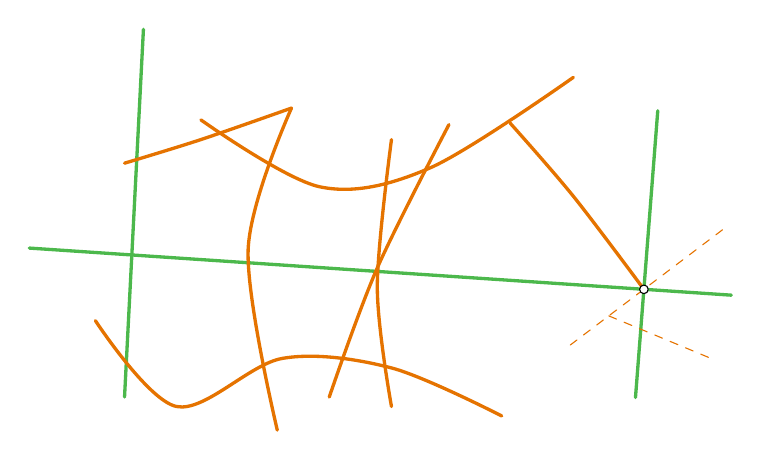
\begin{tikzpicture}[x=1mm,y=1mm,line cap=round,line join=round,font=\scriptsize]
\draw[Lg,very thick] (20.6,-1.2) -- (18.2,-47.9);
\draw[Lg,very thick] (85.92,-11.54) -- (83.09,-47.96);
\draw[Lg,very thick] (6.11,-28.98) -- (95.26,-34.96);
\draw[Or,very thick] plot[smooth, tension=0.55] coordinates {(18.2,-18.2) (27.9,-15.2) (39.4,-11.2)};
\draw[Or,very thick] plot[smooth, tension=0.55] coordinates {(27.9,-12.7) (43,-21.2) (57,-18.8) (75.2,-7.3)};
\draw[Or,very thick] plot[smooth, tension=0.55] coordinates {(39.4,-11.2) (33.9,-29.1) (37.6,-52.1)};
\draw[Or,very thick] plot[smooth, tension=0.55] coordinates {(59.4,-13.3) (50.3,-31.5) (44.2,-47.9)};
\draw[Or,very thick] plot[smooth, tension=0.55] coordinates {(52.1,-15.2) (50.3,-33.9) (52.1,-49.1)};
\draw[Or,very thick] plot[smooth, tension=0.55] coordinates {(67.19,-13.13) (75.2,-22.4) (84.16,-34.22)};
\draw[Or,very thick] plot[smooth, tension=0.55] coordinates {(14.5,-38.2) (24.8,-49.1) (38.2,-43) (52.1,-44.2) (66.1,-50.3)};
\draw[Or,dashed] (74.81,-41.29) -- (94.8,-26.16);
\draw[Or,dashed] (79.7,-37.59) -- (92.7,-43);
\node[opt] at (84.16,-34.22) {};
\end{tikzpicture}
\end{document}
